\section{More Experimental Results}
\paragraph{Prompt Template} For instruction-tuned/aligned LLMs used in the main experiments, we strictly follow their system prompt used during training. Specifically, we list the prompt template used for LLaMa2-7B/13B-Chat, WizardLM-7B, and Zephyr-7B as follows:
\begin{itemize}
    \item LLaMa2-7B/13B-Chat: [INST] <<SYS>> You are a helpful, respectful and honest assistant. Always answer as helpfully as possible, while being safe.  Your answers should not include any harmful, unethical, racist, sexist, toxic, dangerous, or illegal content. Please ensure that your responses are socially unbiased and positive in nature. If a question does not make any sense, or is not factually coherent, explain why instead of answering something not correct. If you don't know the answer to a question, please don't share false information. <</SYS>> \{instruction\}[/INST]
    \item WizardLM-7B: Below is an instruction that describes a task. Write a response that appropriately completes the request. Instruction: \{instruction\} Response:
    \item Zephyr-7B: <|system|> You are a friendly chatbot who always responds in a helpful and detailed manner to the user's questions.</s> <|user|> \{instruction\}</s> <|assistant|>
\end{itemize}
\label{sec:appendix_a}
\paragraph{Extension to GQA/MQA}
We extend existing attention-based eviction policies into GQA and MQA by taking the group-wise averaged attention scores and using it to update the importance score. To verify our extension, we conduct experiments using Zephyr-7B~\cite{tunstall2023zephyr}, an instruction-tuned and aligned version of Mistral-7B~\cite{mistral} on the text summarization task. Specifically, Zephyr-7B employs GQA and has 8 key-value heads and 32 query heads, rendering a 4x replication for each key-value vector pair.

The results are shown in \tabref{table:zephyr}. We can see that, attention-based eviction policies still exhibit better performance compared to Random and StreamLLM, showing that the group-wise average operation can effectively reflect the importance of each token across all query heads within its group.
\paragraph{Results on Larger LLMs} In addition to 7B-scale LLMs, we also examine the effectiveness of RoCo alongside other eviction policies on 13B-scale LLMs. To this end, we conduct a text summarization experiment using LLaMa2-13B-Chat~\cite{llama2} and report the results in \tabref{table:llama213b}. We observe that, given the same KV cache budget, LLaMa2-13B-Chat achieves higher BLEU and ROUGE scores than LLaMa2-7B-Chat. It indicates that a larger model dimension may contain more redundancy in some less informative intermediate activations. This observation is inspiring because it implies that we can preserve more performance when using more powerful LLMs.

\begin{table*}[t!]
    \centering
    \small
    \begin{tabular}{cc|ccccc|ccccc}
    \toprule
    \multicolumn{1}{c}{\multirow{2}{*}{\textbf{Models}}} & \multirow{2}{*}{\textbf{Methods}} & \multicolumn{5}{c}{\textbf{XSum}}         & \multicolumn{5}{c}{\textbf{CNN/DM}}       \\
    \multicolumn{1}{c}{} &              & BLEU & Meteor & R-1  & R-2  & R-L  & BLEU & Meteor & R-1  & R-2  & R-L  \\
    \midrule
    \multirow{6}{*}{Zephyr-7B} & Random &17.0  &39.0  &48.6  &25.2  &34.4  &22.8  &43.2  &54.5  &29.0  &36.1  \\
                         & StreamLLM   &12.0  &35.0    &45.1 &19.3  &29.0  &20.2  &41.2    &51.8  &26.1  &31.9  \\
                         & ScissorHands &26.6  &48.7    &57.4  &34.3  &44.2  &29.4  &49.1    &60.4  &36.0  &44.0  \\
                         & H$_{\text{2}}$O   &29.6  &49.9    &58.9  &38.3  &47.2  &34.9  &52.3    &63.6  &41.3  &48.4  \\
                         & TOVA         &16.8  &40.7    &50.5  &24.6  &34.9  &25.5  &45.8    &57.5  &32.2  &38.6  \\
                         & RoCo         &\textbf{33.6}  &\textbf{54.9}    &\textbf{62.6}  &\textbf{42.4}  &\textbf{50.4}  &\textbf{36.6}  &\textbf{53.8}    &\textbf{64.6}  &\textbf{42.6}  &\textbf{50.0}  \\
    \bottomrule
    \end{tabular}
    \caption{Performance of Zephyr-7B using different eviction policies on abstractive text summarization tasks at 0.5 KV cache rate.}
    \label{table:zephyr}
\end{table*}
\begin{table*}[t!]
    \centering
    \small
    \begin{tabular}{cc|ccccc|ccccc}
    \toprule
    \multicolumn{1}{c}{\multirow{2}{*}{\textbf{Models}}} & \multirow{2}{*}{\textbf{Methods}} & \multicolumn{5}{c}{\textbf{XSum}}         & \multicolumn{5}{c}{\textbf{CNN/DM}}       \\
    \multicolumn{1}{c}{} &              & BLEU & Meteor & R-1  & R-2  & R-L  & BLEU & Meteor & R-1  & R-2  & R-L  \\
    \midrule
    \multirow{4}{*}{LLaMa2-13B$_{\text{Chat}}$} & Random &14.9  &27.7  &30.0  &17.9  &24.5  &9.0  &18.8  &22.3  &11.7  &15.1  \\
                         & StreamLLM   &14.7  &35.7    &41.7 &19.8  &31.2  &26.0  &43.1    &53.2  &30.4  &36.6  \\
                         & H$_{\text{2}}$O   &38.3  &55.9    &61.0  &44.5  &53.4  &38.4  &52.5    &62.3  &42.6  &48.6  \\
                         & RoCo         &\textbf{45.8}  &\textbf{62.2}    &\textbf{66.6}  &\textbf{51.5}  &\textbf{59.3}  &\textbf{41.4}  &\textbf{54.1}    &\textbf{65.1}  &\textbf{47.0}  &\textbf{53.0}  \\
    \bottomrule
    \end{tabular}
    \caption{Performance of LLaMa2-13B-Chat using different eviction policies on abstractive text summarization tasks at 0.5 KV cache rate.}
    \label{table:llama213b}
\end{table*}
\begin{table}[h]
    \centering
    \small
    \begin{tabular}{cccc}
    \toprule
    \textbf{Block Size} & \textbf{BLEU} & \textbf{ROUGE-2} & \textbf{Speed up} \\
    \midrule
    1                   & 26.5          & 35.4            & 1.0x              \\
    2                   & 26.6          & 35.4             & 2.0x              \\
    4                   & 26.5          & 35.4             & 4.0x              \\
    8                   & 26.9          & 35.8             & 8.0x              \\
    16                  & 26.4          & 35.4             & 16.0x             \\
    \bottomrule
    \end{tabular}
    \caption{Performance of Zephyr-7B on text summarization using RoCo. Larger block size only leads to a slight performance decline while significantly speed-up the prefilling stage.}
    \label{table:block}
\end{table}

\section{More Results on Block-wise Eviction} 
\label{sec:appendix_b}
To accelerate key-value constrained prompt encoding, we extend the per-token evict-and-encode scheme to a block-wise manner. We report results on text summarization with various block sizes using Zephyr-7B in \tabref{table:block}. With a larger block size, more tokens are evicted with less reliable importance scores, thereby resulting in some influential tokens being wrongly evicted. Nevertheless, the performance drop is tolerable given the significant speedup of prompt encoding, especially when confronted with long-context tasks~\cite{liu2023lost,longbench,leval}.
\section{Case Study} 
\label{sec:appendix_c}
To obtain a straightforward impression on the generation quality when RoCo is applied for key-value constrained inference, we present responses generated by LLaMa2-7B-Chat given the instruction ``\textit{What are the names of some famous actors that started their careers on Broadway?}''. The responses at different KV cache budget are shown in \figref{fig:case_study}. At 0.3 KV cache budget rate, RoCo generates a response containing the same actor/actress names as the one conditioned on a full KV cache, demonstrating the commendable ability of RoCo to selectively retain useful key-value states and maintain coherent generation.
\begin{figure*}[t!]
	\centering
	\scalebox{0.54}{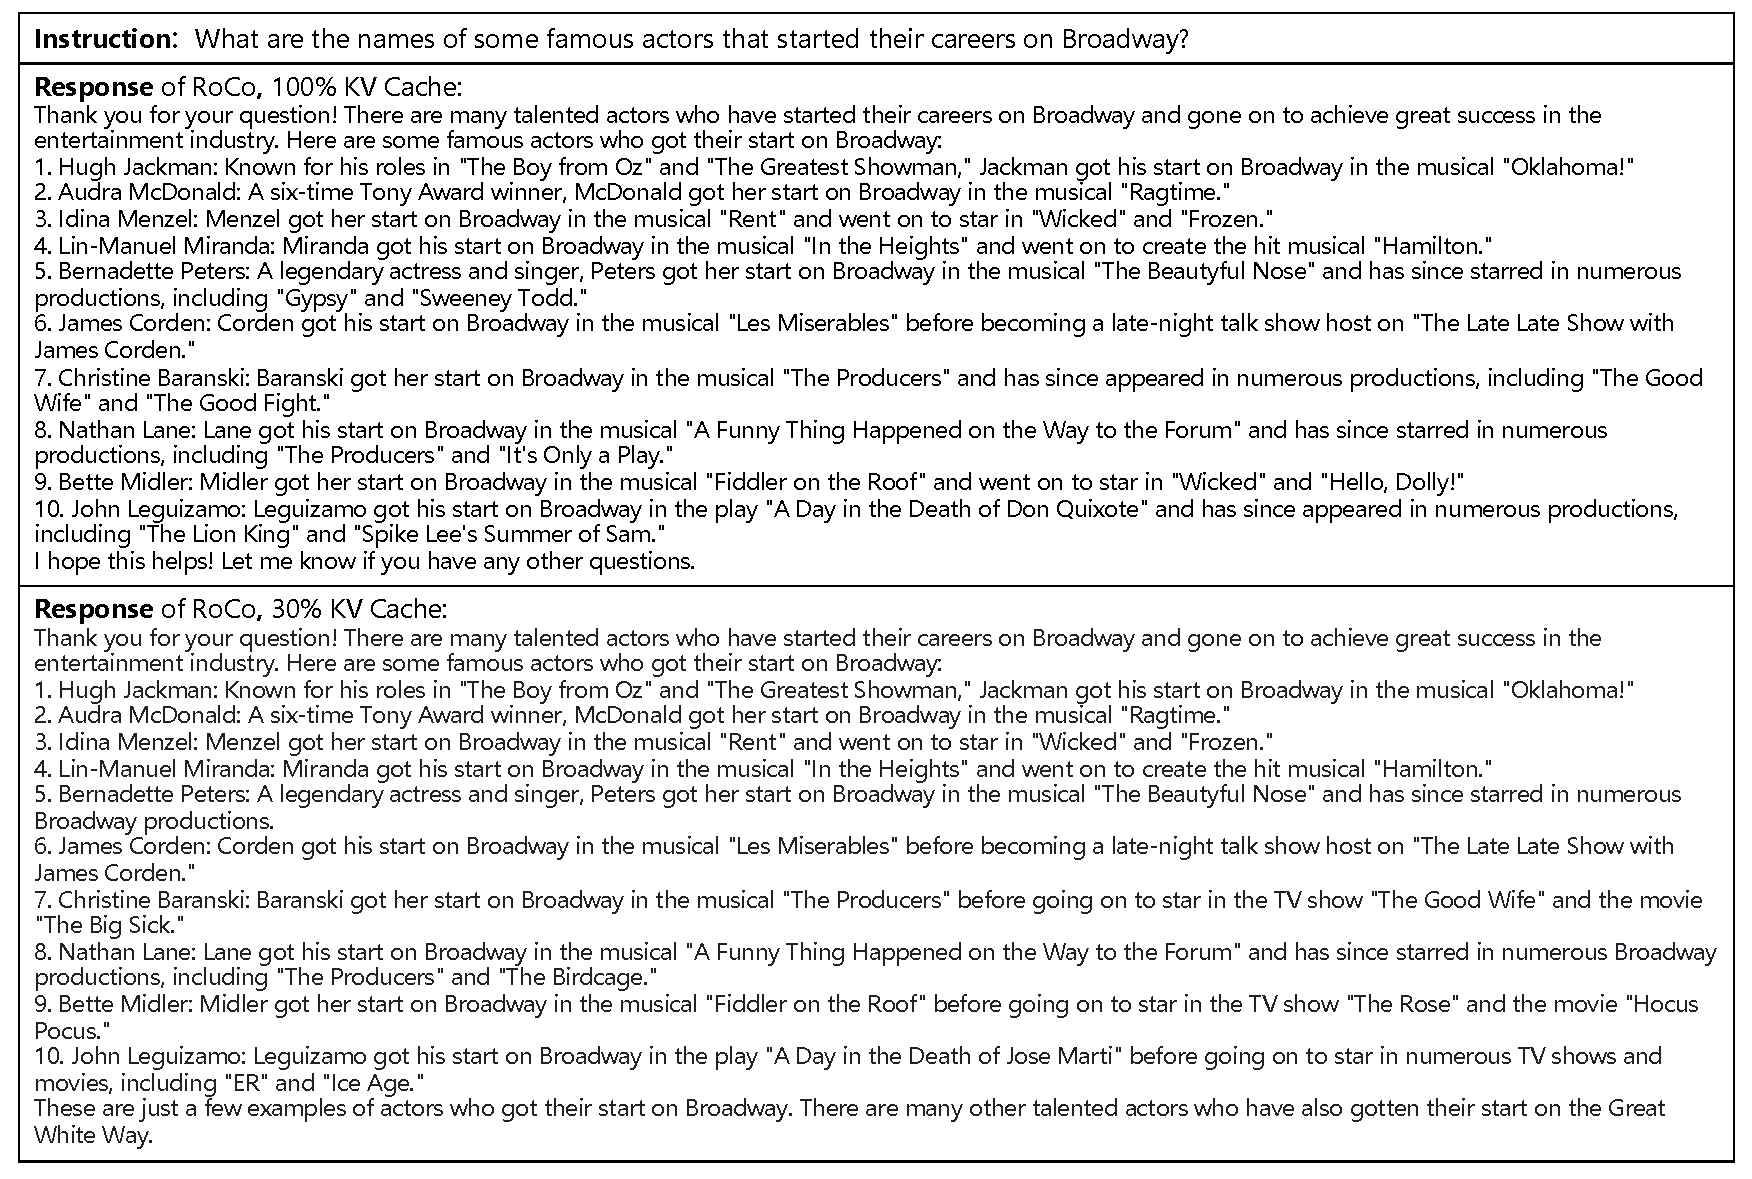
\includegraphics{./figures/case_study.pdf}}
    \caption{Case study of LLaMa2-7B-Chat generated response given a specific instruction. The response generated with 30\% KV cache using RoCo retains almost all content in the original response.}
	\label{fig:case_study}
\end{figure*}